\chapter{Adiabatic Quantum Computing}
\label{chap:aqc}

\section{The Adiabatic Theorem}

The central idea of Adiabatic Quantum Computation (AQC) is solving problems by finding the ground states of specially constructed Hamiltonians.\cite{farhi}  Ground state relaxation is a form of analog computing where we rely on physics to do the calculating for us: we set up a physical system so that the ground state is the solution to our problem and let the system evolve.  Generally speaking, we expect that classical or quantum systems will still take exponentially long to reach this desired ground state for NP-hard problems.\cite{aaronson}
By starting the system in an easy to prepare state (e.g. ferromagnetically aligned) and then evolving adiabatically into our prepared problem state AQC uses the \emph{adiabatic theorem} to (hopefully) avoid this exponential delay.

The adiabatic theorem states that if a system is initially prepared in the ith energy level, and the Hamiltonian is evolved according to the adiabatic condition, the system will remain in the ith state after the evolution.  The adiabatic condition is:

\begin{equation}
	\left | \frac{1}{\omega_{fi}}\frac{\partial}{\partial t} \braket{\psi_f | \hat{V}(t) | \psi_i} \right | << |E_f - E_i|
\end{equation}

where $E_i$ and $E_f$ are the energies of the initial and final states, $\hat{V}(t)$ is the time dependant part of the Hamiltonian and $\omega_{if} = \frac{E_f - E_i}{\hbar}$ is a convenient variable.  This (FIXME missing! also maybe put the derivation in an appendix) derivation due to \cite{zettili}.  When the adiabatic condition is satisfied, the probability of transition from state $i$ to state $f$ is zero.

So if the speed at which the Hamiltonian changes (the derivative term) is slow enough, and the gap between the initial state and the other states ($E_f - E_i$) is large enough, then the system won't transition into a new state.  

\section{Finding a Problem Hamiltonian}
\label{sec:prob_ham}
While in principle there are an unlimited number of ways to construct a Hamiltonian whose ground state encodes the solution to a computation, our method is to use an N-particle Hamiltonian of the form

\begin{equation}
	\ham_f = \sum_{i} h_i \sigma_i^Z + \sum_{i < j} J_{ij} \sigma_i^Z\sigma_j^Z 
\end{equation}
where $\sigma_i^Z$ is the z-pauli matrix of the ith particle and $h_i$ and $J_{ij}$ are the parameters of the Hamiltonian.  This 2-local Hamiltonian corresponds to a graph structure, where each particle is a vertex and each non-zero $J_{ij}$ is an edge, while non-zero $h_i$s can be represented as edges to a constant ``field'' spin.

Our problem of finding a suitable Hamiltonian is now reduced to finding a set of $h$'s and $J_{ij}$'s such that our desired solution is encoded in the ground state.  We do this by breaking our problem down into sub-problems and finding Hamiltonians for these easier sub-problems, and then reassembling these smaller Hamiltonians into the final problem Hamiltonian using the gluing theorem.\cite{gluing}

Figure \ref{fig:nand_graph} shows a Hamiltonian graph describing the $h_i$'s and $J_{ij}$'s to encode the logic of a NAND gate.  Because NAND's are universal for computation, combining this graph with the gluing theorem allows us to encode the evaluation of any computable function into the ground state of a Hamiltonian of the general form we described above.  

\begin{figure}
	\begin{center}
	\scalebox{0.5}{
		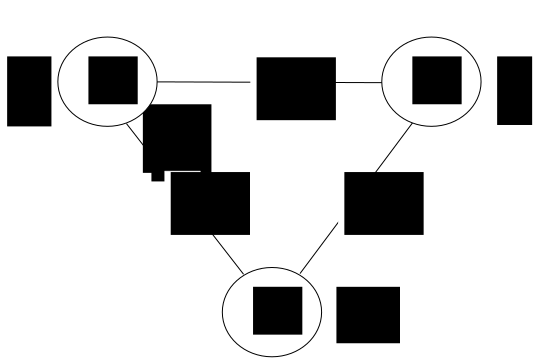
\includegraphics{img/nand.eps}
	}
\end{center}
	\caption[\texttt{NAND} Graph]{Graphical representation of the Hamiltonian implementing the logic of a \texttt{NAND} gate.  Each of the vertices is a spin and the number inside is the field value on that spin; each edge is the coupling value between the respective vertices.  The top two spins are the input spins, while the bottom is the output.  Each ground state of this Hamiltonian enforces the logic $C = \neg(A \wedge B)$.}
	\label{fig:nand_graph}
\end{figure}


We don't expect this encoding using NANDs glued together to be either optimal in the sense of using fewest spins or couplings, or to be asymptotically faster than an equivalent classical circuit.  We have no general solution for the first problem; each computational problem we want to encode efficiently requires it's own bespoke encoding.  
To solve the second problem we take advantage of the fact that quantum mechanics is time-reversible: which variables are output and which are input is arbitrary.  
Thus if we have a solution in mind for a given problem we can simply encode the Hamiltonian ``backwards'' and recover answers that would lead to our initial solution.  For NP problems, where verifying a solution is in P, we can thus write a verification circuit with a solution of \texttt{true} and find the inputs to our NP problem.
It seems reasonable that a circuit for multiplication will be evaluable in polynomial time; because factoring can be solved with the same circuit, it is not inconceivable that a factoring circuit could be evaluable in polynomial time as well.

Our approach to solving NP problems is thus:
\begin{itemize}
	\item Construct a circuit to verify a candidate solution (for satisfiability this would be evaluation of the clauses; for factoring this would be a multiplication circuit)
	\item Clamp the ``output'' spins to their required values (for a satisfiability problem this would be all output spins \texttt{true}; for a factoring problem this would be the number to factor)
	\item Run the adiabatic computer and read off the ``input'' spins
\end{itemize}

Clamping is the process whereby we take a Hamiltonian containing variables $s_i$ as well as the variable $c$, and modify the Hamiltonian so that the variable to be clamped ($c$) is no longer present.  The field term on $c$ is multiplied by the value that $c$ is to be clamped to ($v = \pm1$), and the ground state energy is shifted by that value.  Then each coupling which connected $c$ to another variable is removed, and the field on that variable is adjusted by the value of the coupling that was removed multiplied by $v$.  The resulting energy structure is the same as the initial Hamiltonian, but as if there was an infinitely large field on $c$ holding it either up or down.  This procedure can be repeated for more than one spin.

\section{Adiabatic Evolution}
Once we have a Hamiltonian whose ground state encodes the problem we would like to solve, we need to set up the evolution.  The Adiabatic Theorem lets us transition from the ground state of one Hamiltonian to another, so we need an initial Hamiltonian.  In general almost any Hamiltonian which we know the ground state of will work, and we know that the choice of initial Hamiltonian affects the evolution in ways we can't predict.  For simplicity however, we use the following initial Hamiltonian:
\begin{equation}
	\ham_i = \sum_i^N B \sigma_i^x
\end{equation}
where $B$ is some large constant.  This Hamiltonian has as it's ground state all the spins pointed along the (negative) x-axis (or equivalently, an equal superposition of $\ket{\pm z}$).  This is easy to prepare by applying a large magnetic field along the negative x direction.
Once we've assembled both our initial and final Hamiltonians, we can conduct the evolution.  We call the total Hamiltonian $H_{tot}$, and it is simply the sum of the initial and final Hamiltonian:

\begin{equation}
	\ham_{tot} = A(t)\ham_i + B(t)\ham_f
\end{equation}

where $f$ and $g$ are dimensionless functions of time such that $A(0) = B(T) = 1$ and $A(T) = B(0) = 0$ where $T$ is the final annealing time; this ensures that at $t = 0$ the Hamiltonian is equal to $H_i$ and at $t = T$ the Hamiltonian is equal to $H_f$.  Then the functions $A$ and $B$ describe the \emph{evolution path}.  Combining the evolution path with the speed at which the Hamiltonian is changing (or just the speed), that is $\frac{\partial A}{\partial t}$ and $\frac{\partial B}{\partial t}$, gives us the evolution trajectory.  

Given a ground state of $\ham_{tot}$, $\ket{\psi_{gs}}$, the \emph{fidelity} is the probability of measuring $\psi_{gs}$, or $|\braket{\psi_{gs}|\ham_f|\psi_{gs}}|^2$.  If there are $N$ correct answer to our computation, and thus $\ket{\psi_N}$ degenerate ground states, the fidelity is defined as

\begin{equation}
	F = \sum_{i=0}^N \braket{\psi_i|\ham_f|\psi_i}
\end{equation}

For a perfectly annealed system, the fidelity should go to one as the annealing time increases.  Since any real annealing will not be in the infinite anneal time limit, in practice our fidelity values are restricted to be $\leq 1$.  The closer the fidelity is to 1, the more likely our computation is to succeed.

For a purely quantum mechanical system described by the Hamiltonian $\ham_{tot}$, the evolution trajectory completely determines the fidelity.
The simplest and most obvious trajectory is $A(t) = 1 - t/T$ and $B(t) = t/T$ at a constant speed, or a straight line path through Hamiltonian space.
Obviously the gap must go to zero as both $A$ and $B$ approach zero; in the absence of any Hamiltonian all states have equal energy.  Likewise scaling $A$ and $B$ by a uniform factor scales the gap by the same factor.  So if we imagine a heightmap of the gap as a function of $A$ and $B$, there is a minimum at $(A=0,B=0)$ and the gap increases along both axes.  
There is no particular reason that a straight line from $(1,0)$ to $(0,1)$ should maximize the fidelity; indeed we expect that some more complicated curve through Hamiltonian space, potentially including dynamically changing the evolution speed, will give the best results.
Unfortunately, the physical \texttt{VESUVIUS} machine has a fixed trajectory, with the path and the evolution speed predetermined.  This trajectory is shown in Figure \ref{fig:trajectory}.
This means that any results we measure are not only specific to machines of the specific type employed by D-Wave, but that even future models of theirs might have very different characteristics.  This is especially true a hypothetical future model that would allow changing the annealing schedule to suit the problem, or even better dynamically changing the annealing schedule on the fly.
